\begin{table*}[!htbp]
\centering
\caption{Composition of the Datasets}
\label{tab:dataset_composition}
\resizebox{\linewidth}{!}{%
    \begin{tabular}{l|ccc|ccc|ccc}
    \multirow{2}{*}{{\bf Dataset}} & \multicolumn{3}{c|}{\bf Train} & \multicolumn{3}{c|}{\bf Test known} & \multicolumn{3}{c}{\bf Test unknown} \\
     & {\bf Live} & {\bf Contacts} & {\bf Printouts} & {\bf Live} & {\bf Contacts} & {\bf Printouts} & {\bf Live} & {\bf Contacts} & {\bf Printouts} \\ \hline\hline
    Clarkson & 2,469 & 1,122 & 1,346 & 1,485 & 765 & 908 & 638 & 494 & 144 \\ \hline
    IIITD-WVU & 2,250 & 1,000 & 3,000 & -- & -- & -- & 702 & 701 & 2,806 \\ \hline
    Notre Dame & 600 & 600 & -- & 900 & 900 & -- & 900 & 900 & -- \\ \hline
    Warsaw & 1,844 & -- & 2,669 & 974 & -- & 2,016 & 2,350 & -- & 2,160 \\ \hline\hline
    Combined & 7,163 & 2,722 & 7,015 & 3,359 & 1,665 & 2,924 & 4,590 & 2,095 & 5,110 \\
    \end{tabular}%
    }
\end{table*}

\subsection{Datasets}
\label{sec:dataset}

Our work was performed on datasets made available in the Iris Liveness Detection Competition 2017 \cite{Yambay2017}. There is one set from each of four universities involved --- Clarkson University, Warsaw University of Technology, IIITD-WVU and University of Notre Dame.

The Clarkson dataset \cite{Yambay2014, Yambay2015, Yambay2017} contains images of live irises, textured contact lenses, and iris printouts. The Warsaw dataset \cite{Yambay2017} comprises images of live irises and iris printouts. 
The Notre Dame dataset \cite{Doyle2015} contains images of live irises without textured contact lenses and of irises wearing textured contact lenses. Finally, the IIITD-WVU dataset \cite{Kohli2013, Gupta2014, Yadav2014, Kohli2016} contains images of live irises, textured contact lenses, iris printouts, and printouts of textured contact lenses.
Table \ref{tab:dataset_composition} summarizes the composition of the datasets. For some of our experiments, we also formed a merged dataset by combining the four sets, which we will refer to as the ``Combined'' dataset. The original cross-validation partitioning was kept the same in the ``Combined'' dataset.

\begin{figure*}[!htb]
    \centering
    \begin{subfigure}[b]{0.99\linewidth}
        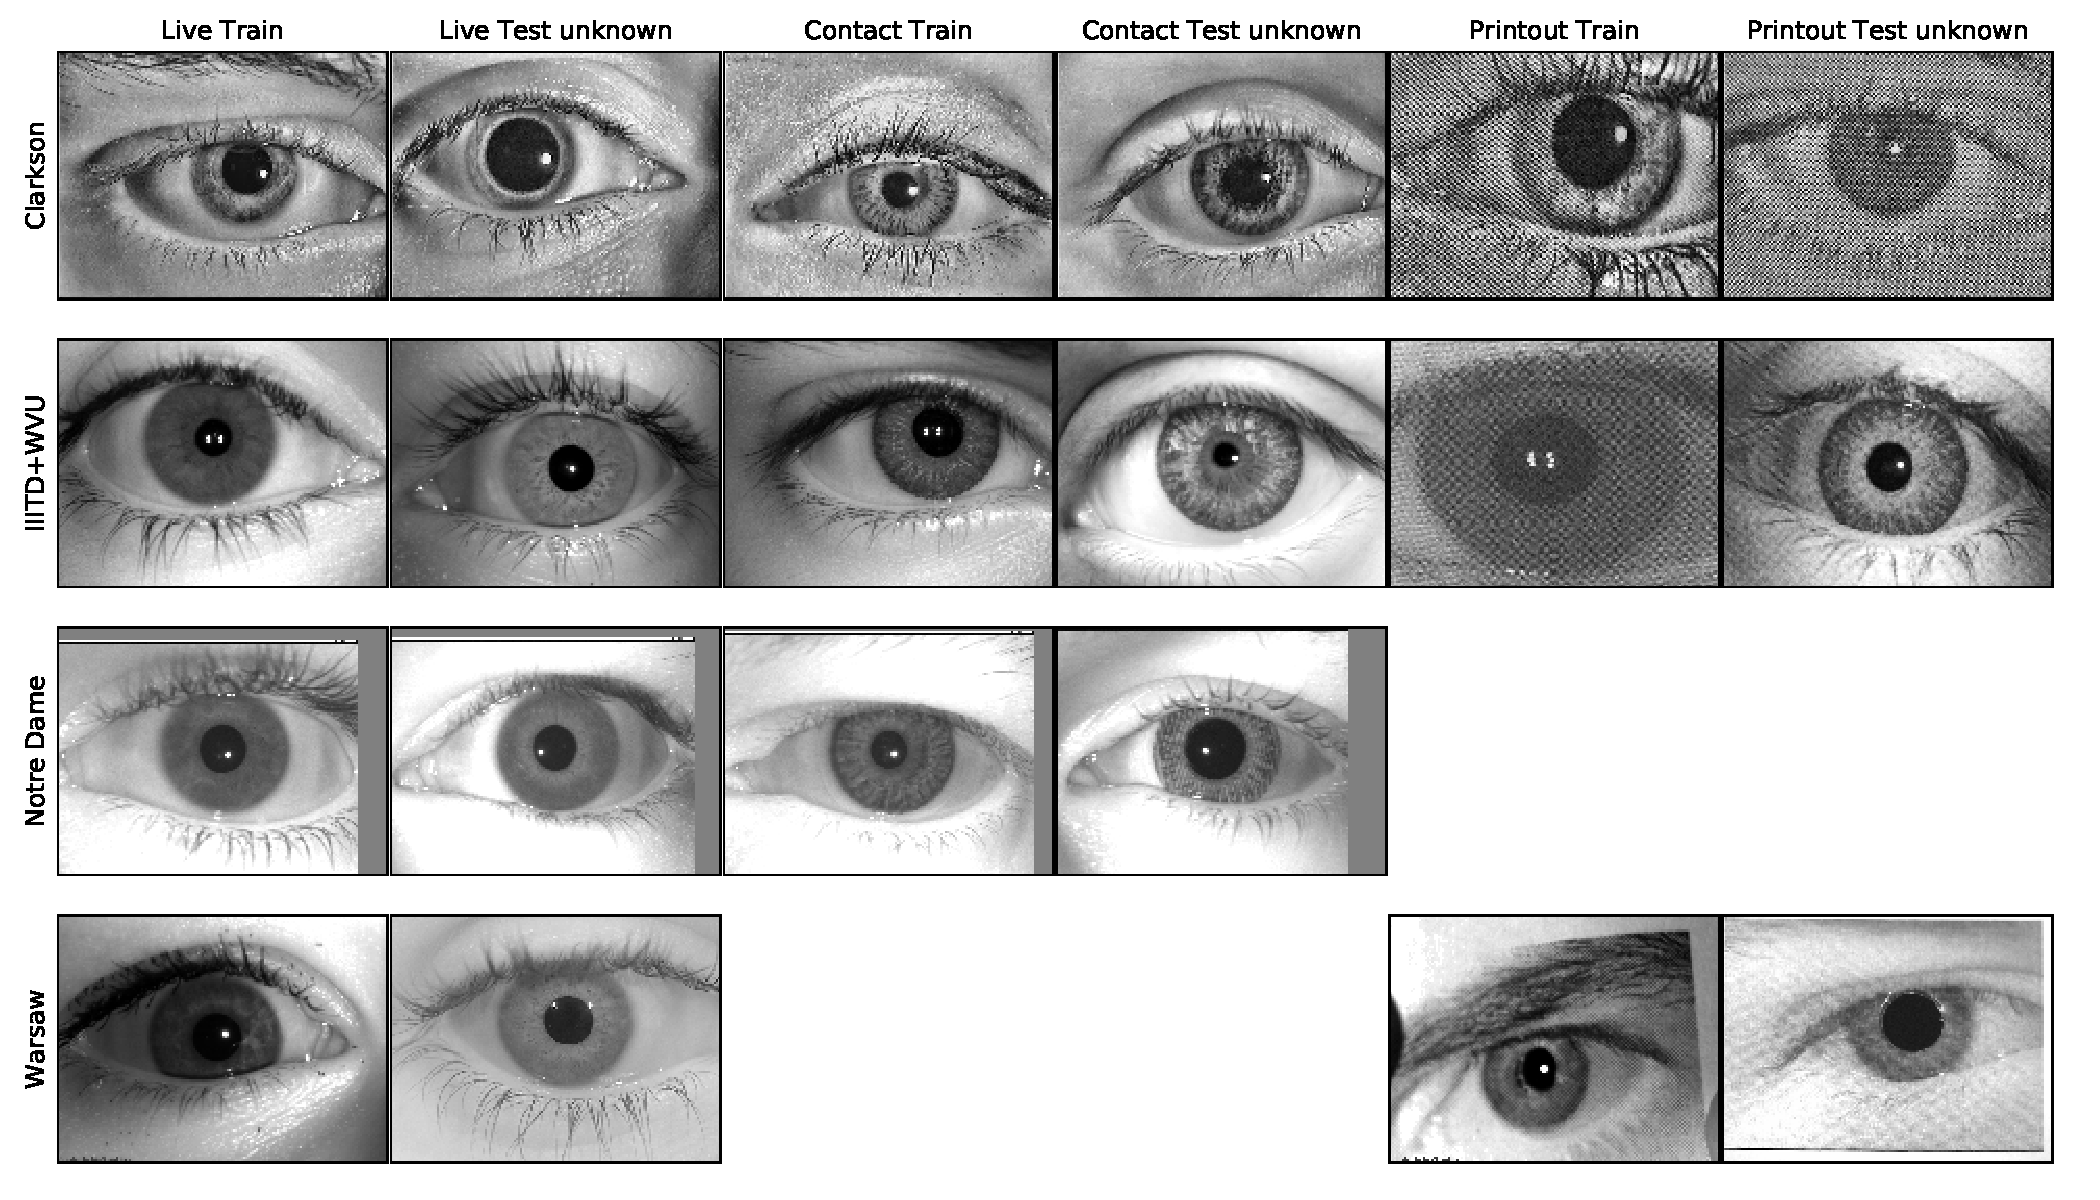
\includegraphics[width=\linewidth, 
                         trim=0.4cm 0.5cm 0.8cm 0.3cm,clip]{imgsamples.pdf}
    \end{subfigure}
    \caption{Image samples from all datasets, from the \emph{train} and \emph{unknown} partitions. The difference between train and unknown images, especially in the case of attacks, illustrates situations where classifiers commonly fail.}
    \label{fig:img_samples}
\end{figure*}

Each dataset is composed of a \emph{train} partition, made available to the participants to facilitate training their algorithms, and a \emph{test} partition, not distributed before the competition was ended, and used by the organizers to evaluate the submissions. LivDet-Iris 2017 co-organizers marked their test samples to form two groups of images. In the first group, referred to as \emph{test known}, both live images and images of artifacts had the same ``known'' properties as train samples. The images belonging to a second group, \emph{test unknown}, have different, or ``unknown'', properties than pictures included in the train subsets. Competition organizers applied different strategies when producing the \emph{test unknown} samples. Clarkson University included visible-light image printouts and new patterns of textured contact lenses, Warsaw University of Technology used different equipment to prepare and photograph iris printouts. The images of patterned contact lenses offered by University of Notre Dame are of different brands than those in the train set. Finally, the whole test partition of the IIITD-WVU benchmark is considered as \emph{test unknown}, since it was collected by a different institution (WVU) than the train set (IIITD), by a different sensor, and included outdoor acquisitions. Figure \ref{fig:img_samples} shows sample images of each dataset.

To keep our evaluation protocol compliant with LivDet-Iris 2017, training of our methods uses solely pre-defined training partitions of the datasets, while the final performance is estimated both on the \emph{test known} and \emph{test unknown} partitions.

